\chapter{Evaluation} \label{ch:evaluation}
We have used a machine learning toolkit named as GRT to recognize hand gestures using skeletal points tracking algorithm and Adaptive Naive Bayes classifier (ANBC) for classification and prediction. 

The classifier is based on a statistical model of x,y,z coordinate positions of static hand gestures and provides a likelihood measure for recognized gesture. Furthermore, the gesture recognition pipeline uses two post processing modules such as Class Label Filter and Class Label Change Filter to exclude lower frequent spikes in the prediction results and trigger an output only when there is a change in prediction.

In this chapter, we present the experiments carried out to evaluate and validate our system to recognize hand gestures using skeletal points. The goal is to demonstrate the effectiveness of the classifier and to evaluate its potential for real time input at 30 fps. In the classification phase, input samples are normalized using Min-Max Scaling and Null Rejection is enabled to detect non-gestures. Therefore, the evaluation consists of computing the prediction accuracy for various null rejection coefficient and compare it with other supervised learning classifiers such as Support Vector Machine (SVM) and Minimum Distance (MinDist).

\section{Mean and Standard Deviation}
ANBC is a supervised learning algorithm that can be used to classify any type of N-dimensional signal. It fundamentally works by fitting an N-dimensional Gaussian distribution to each class when it is trained.

During the training phase, first all the input samples are normalized using Min-Max Scaling with the range from 0 to 1 and then GRT computes mean $\mu$ and standard deviation $\sigma$ to create a model for each class. During the prediction phase, it basically computes the maximum a posterior probability of an input vector belonging to any of the trained class. Figure \ref{fg:ev:mean} shows the mean positions of left and right hand for every gesture. Table \ref{tb:ev:mean} and \ref{tb:ev:sd} show mean and standard deviations of the labeled training data of all the five classes. 

\section{Classification and Prediction}
Our gesture recognition pipeline is trained with 11918 input samples of 6 dimensional vector for 5 classes. Class 1,2,3,4,5 are mapped to Walk, Turn Right, Turn Left, Move Right, Move Left gestures respectively. We have carried out experiments to evaluate the classification, prediction and post processing efficiency of our system. Graph \ref{ev:test:prediction} show change is positions of left and hand in Cartesian coordinates while test data was recorded and corresponding prediction for every input sample.

Test data consists of 1400 samples which are recorded under supervised arrangement. Input vectors that is not containing left and right hand are removed from the test data. Furthermore, input vectors which were recorded when the hand is at the field of view of the camera are also excluded. A program was implemented with GRT to read all the test data and execute prediction on every input sample and then results are stored to CSV file. Finally results are plotted using MATLAB.

Prediction results shown in the graph \ref{ev:test:prediction} frequently falls down to Class Label 0 that is reserved for non-gestures. Non-gestures are detected with the help of Null Rejection thresholds. Therefore, this prediction is based on normalized classification data for Adaptive Naive Bayes classifier with Null rejection coefficient of 1.0.

\section{Prediction Accuracy Vs Null Rejection Accuracy} \label{sec:ev:accuracy}
Classifiers of GRT offers various customization that could produce different results for the same test data. Accuracy of a gesture recognition system does not depend only on th precise predictions of trained gestures,  but also differentiating them from unintended hand gestures. Graph \ref{ev:accuracy:anbc} shows the prediction and null rejection accuracies of Adaptive Naive Bayes Classifier (ANBC). Graph shows the accuracies of 5 trained gestures and a non-gesture. Non-Gesture data was recorded with both the hands are pointing downwards. GRT allows us to set null rejection coefficient for the classifier and therefore, graph contains the dataset of accuracies with null rejection coefficients range from 0 to 10.

Graph \ref{ev:accuracy:anbc} shows that increase in null rejection coefficient causes an increase in the accuracy of trained gestures, however, causes a decrease in the accuracy of non-gesture. Therefore, it is optimal to use a null rejection coefficient of 2.0 with ANBC.

Graph \ref{ev:accuracy:svm} shows prediction results of Support Vector Machine classifier with RBF Kernel. It is apparent that accuracy of trained gestures are consistently above 95 percent. However, null rejection accuracy is constantly lesser than 10 percent, thus, denoting that SVM is not useful in our case, because the robot should not execute any unintended commands.

Graph \ref{ev:accuracy:mindist} shows some interesting results of Minimum Distance classifier with 4 clusters. Graph shows that prediction results are unpredictable as there is increase in null rejection coefficient. However, with coefficient of around 6.3, MinDist shows compromising accuracy above 90 percent for trained gesture and non-gesture. This shows that MinDist is a better alternative to ANBC. 

\begin{table}
	\centering
	\pgfplotstabletypeset [ col sep=comma, every head row/.style={before row=\hline,after row=\hline}, every last row/.style={after row=\hline}, ] {../../data/results/mean.csv}
	\caption{Normalized mean values of 3 dimensions of left and right hand} \label{tb:ev:mean} 
\end{table}

\begin{table}
	\centering
	\pgfkeys{/pgf/number format/.cd,fixed,fixed zerofill,precision=3}
	\pgfplotstabletypeset [ col sep=comma, every head row/.style={before row=\hline,after row=\hline}, every last row/.style={after row=\hline}, ] {../../data/results/sd.csv} \caption{Standard deviations of 3 dimensions of left and right hand} \label{tb:ev:sd} 
\end{table}

\begin{table}
	\centering
		\pgfkeys{/pgf/number format/.cd,fixed,fixed zerofill,precision=3}
	\pgfplotstabletypeset [ 
	col sep=comma, 
	every head row/.style={before row=\hline,after row=\hline},
	every last row/.style={after row=\hline},
	create on use/newcol/.style={
		create col/set list={Precision,Recall,F-measure}
	},
	columns/newcol/.style={string type},
	columns={newcol,0,1,2,3,4},
	display columns/0/.style={column name={}},
	display columns/1/.style={column name={Class 1}},
	display columns/2/.style={column name={Class 2}},
	display columns/3/.style={column name={Class 3}},
	display columns/4/.style={column name={Class 4}},
	display columns/5/.style={column name={Class 5}},
	] 
	{../../data/results/subset-test/anbc2-precision-recall-fmeasure.csv}
	\caption{Precision, Recall and F-Measure calculated by validating 10\% of training dataset. ANBC Classifier trained with Null Rejection coefficient 2.0} \label{tb:ev:confusion} 
\end{table}


\begin{table}
	\centering
	\pgfkeys{/pgf/number format/.cd,fixed,fixed zerofill,precision=3}
	\pgfplotstabletypeset [ 
	col sep=comma, 
	every head row/.style={before row=\hline,after row=\hline},
	every last row/.style={after row=\hline},
	create on use/newcol/.style={
		create col/set list={Non-gesture,Class 1,Class 2,Class 3,Class 4,Class 5}
	},
	columns/newcol/.style={string type},
	columns={newcol,0,1,2,3,4,5},
	display columns/0/.style={column name={}},
	display columns/1/.style={column name={Non-Gesture}},
	display columns/2/.style={column name={Class 1}},
	display columns/3/.style={column name={Class 2}},
	display columns/4/.style={column name={Class 3}},
	display columns/5/.style={column name={Class 4}},
	display columns/6/.style={column name={Class 5}},				
	] 
	{../../data/results/subset-test/anbc2-confusion.csv}
	\caption{Confusion Matrix calculated by validating 10\% of training dataset. ANBC Classifier trained with Null Rejection coefficient 2.0} \label{tb:ev:confusion} 
\end{table}




\clearpage
\begin{figure}
	[h]
	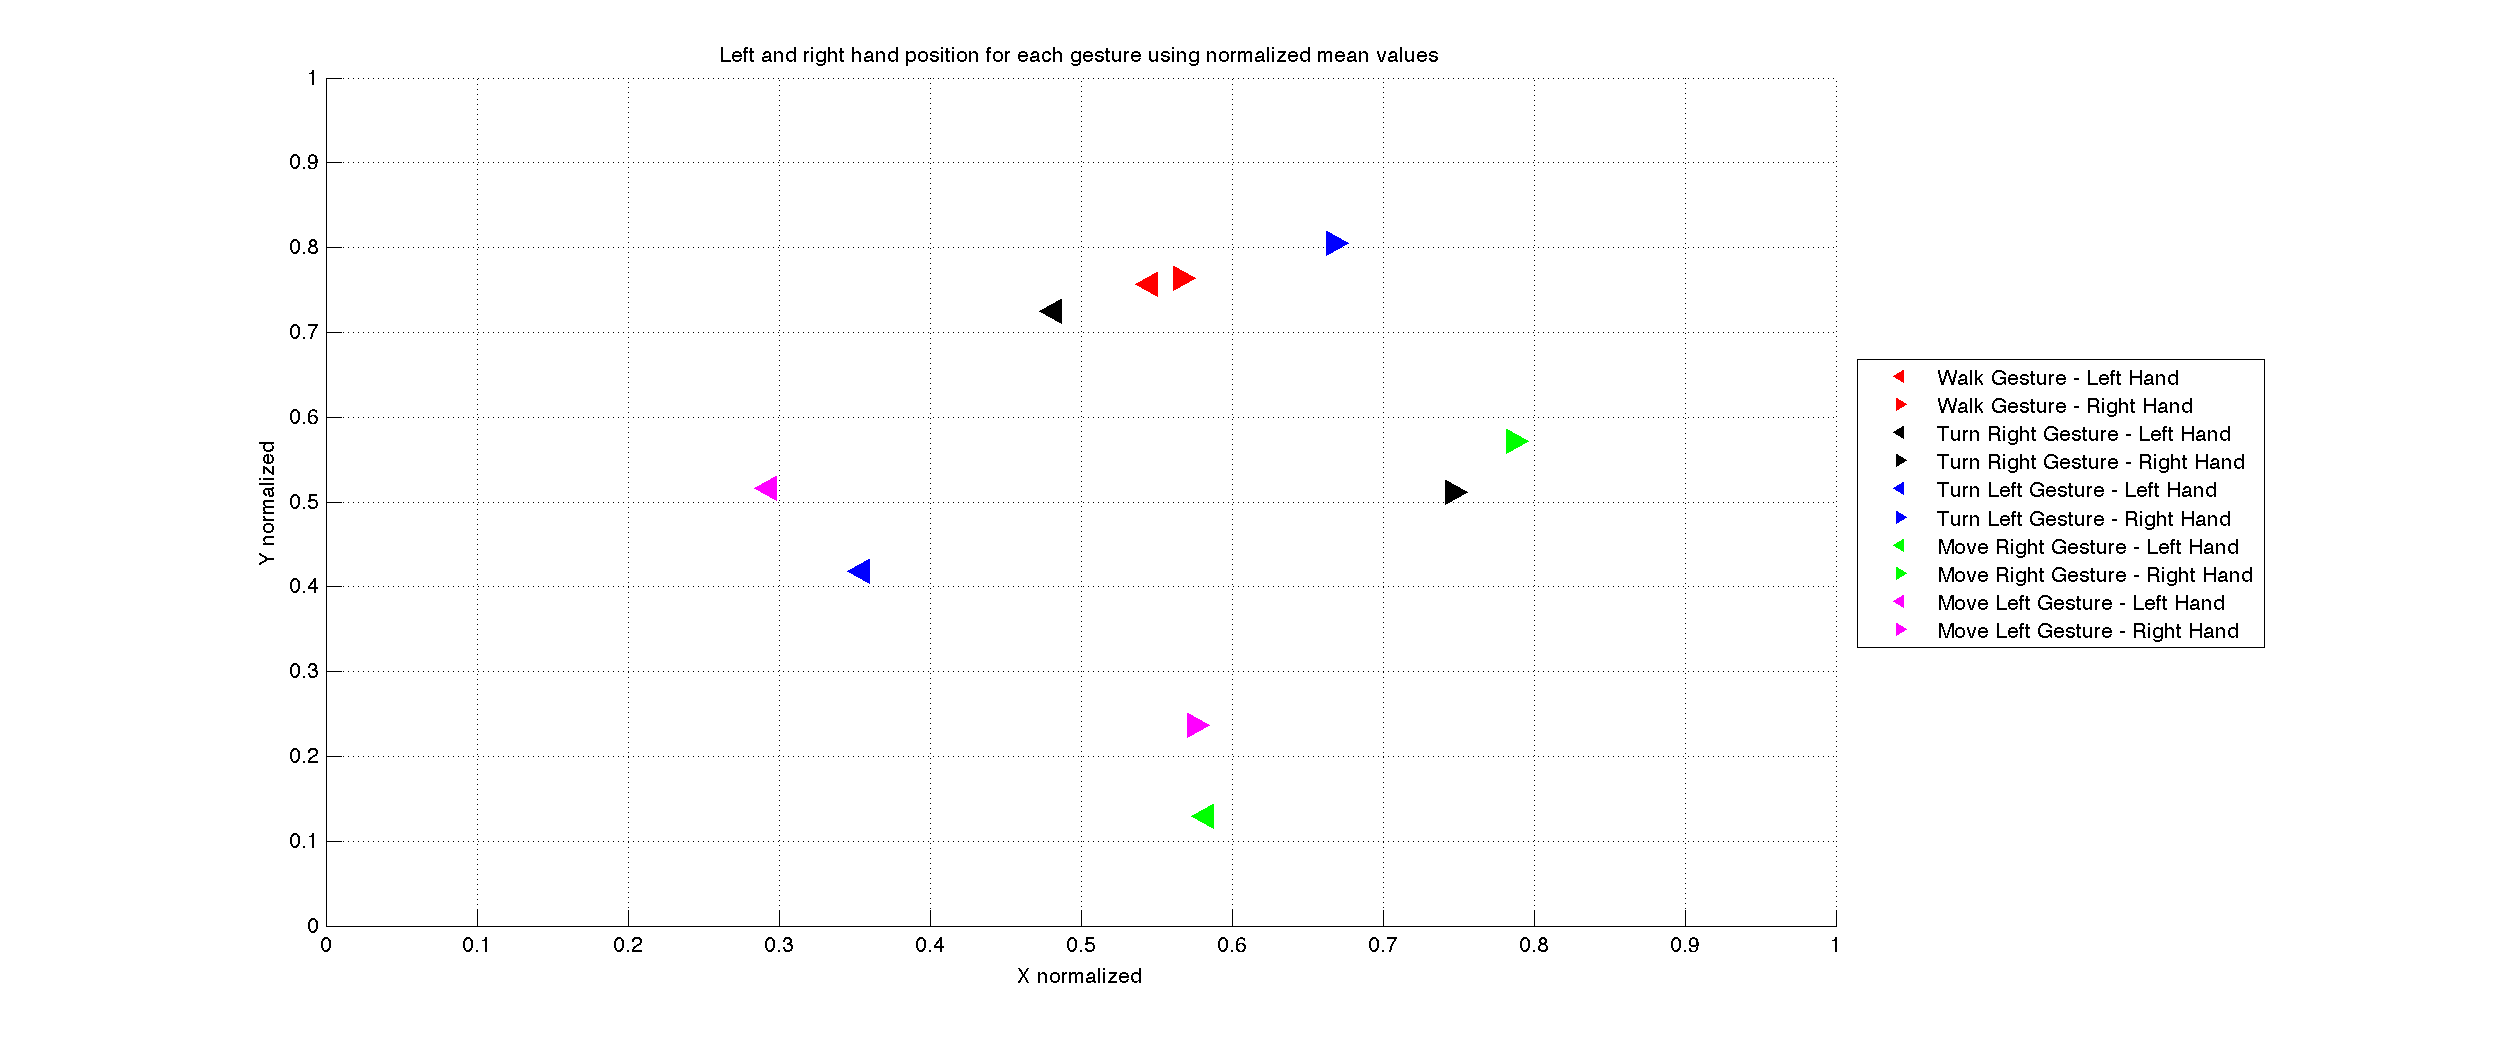
\includegraphics[height=70mm]{/result/train-all-ges-mean.png} \caption{Left and right hand position for each gesture using normalized mean values} \label{fg:ev:mean} 
\end{figure}

\begin{figure}
	[h]
	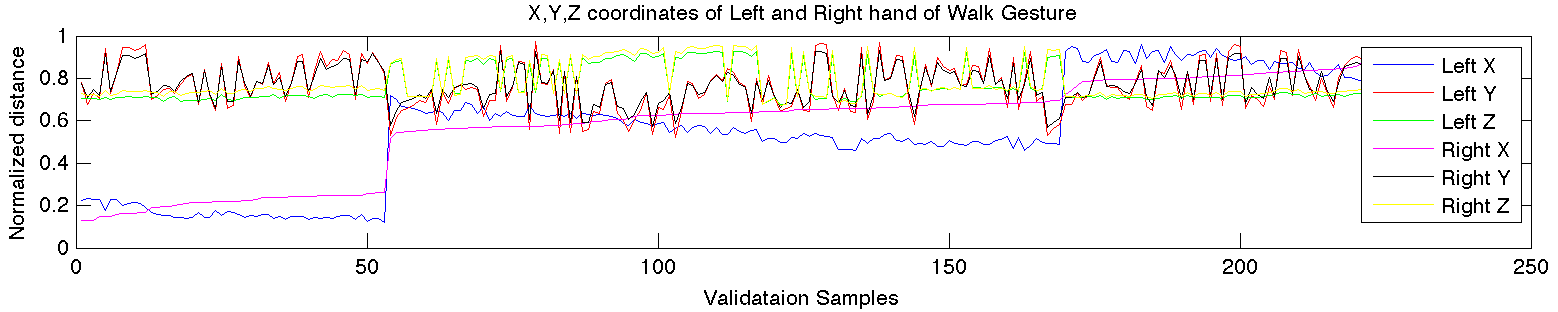
\includegraphics[width=150mm]{/result/test-axis-walk.png} 
\end{figure}
\begin{figure}
	[h]
	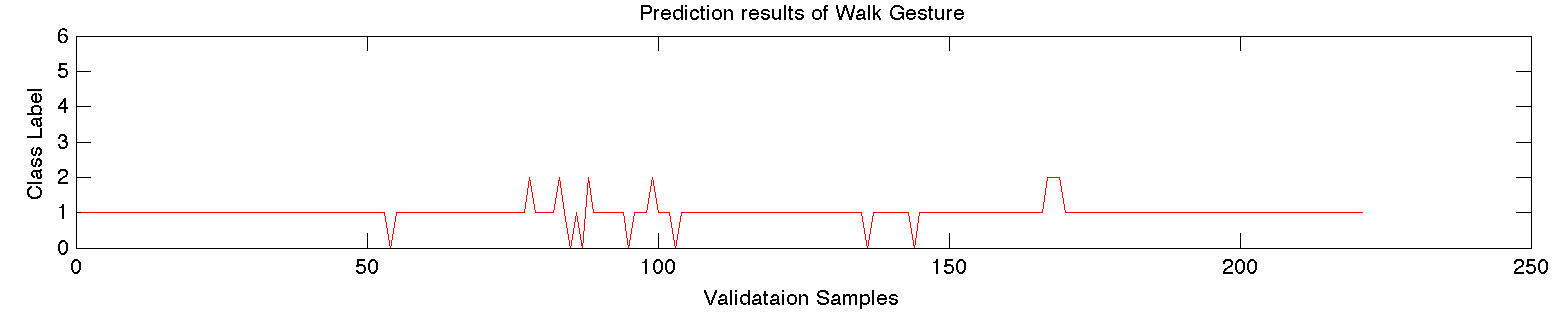
\includegraphics[width=150mm]{/result/test-prediction-walk.png} 
\end{figure}
\begin{figure}
	[h]
	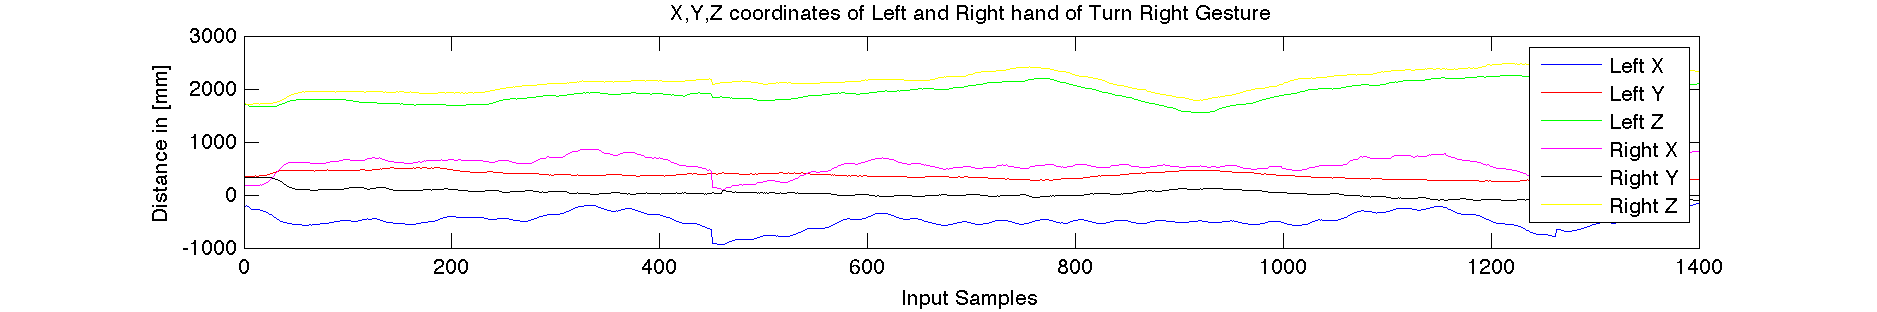
\includegraphics[width=150mm]{/result/test-axis-turn-right.png} 
\end{figure}
\begin{figure}
	[h]
	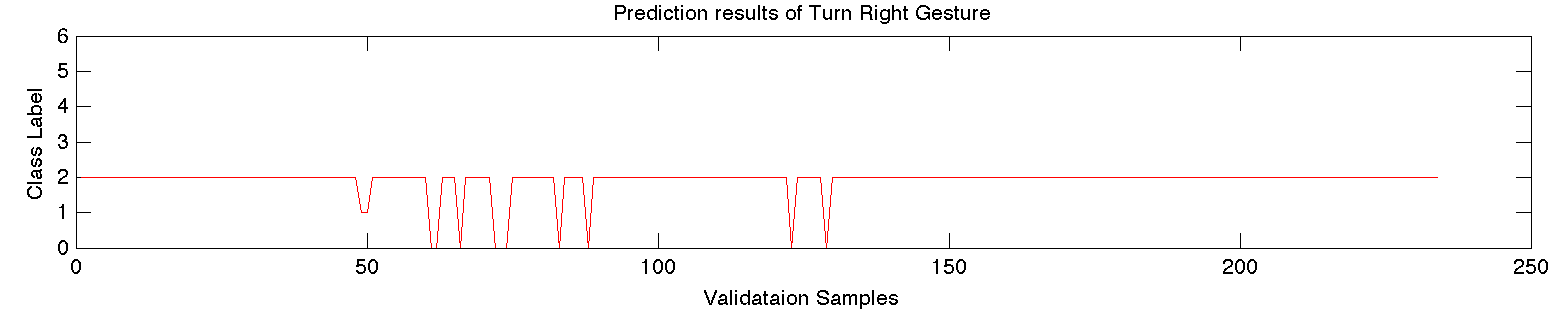
\includegraphics[width=150mm]{/result/test-prediction-turn-right.png} 
\end{figure}
\begin{figure}
	[h]
	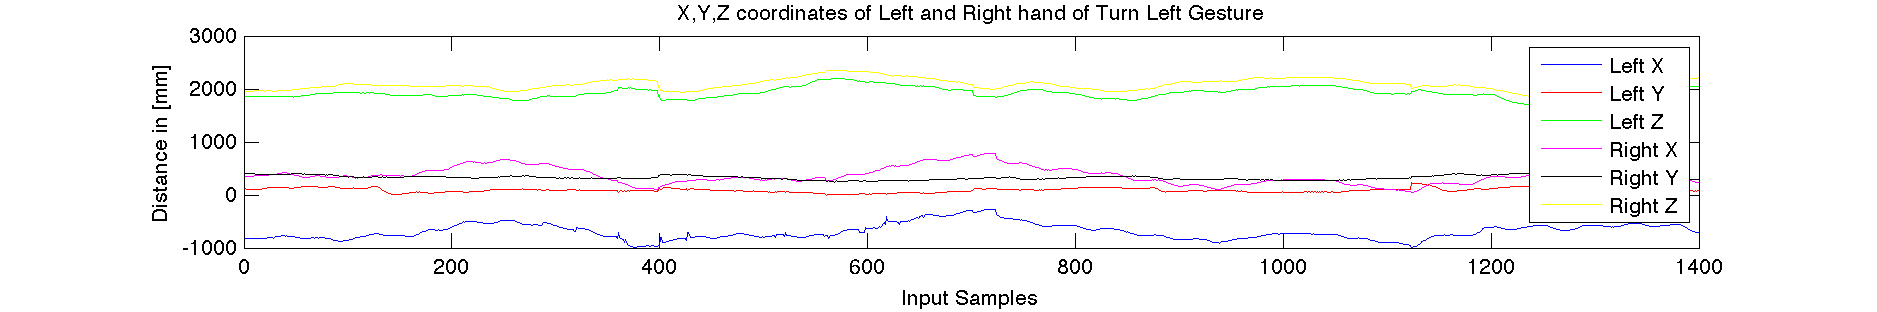
\includegraphics[width=150mm]{/result/test-axis-turn-left.png} 
\end{figure}
\begin{figure}
	[h]
	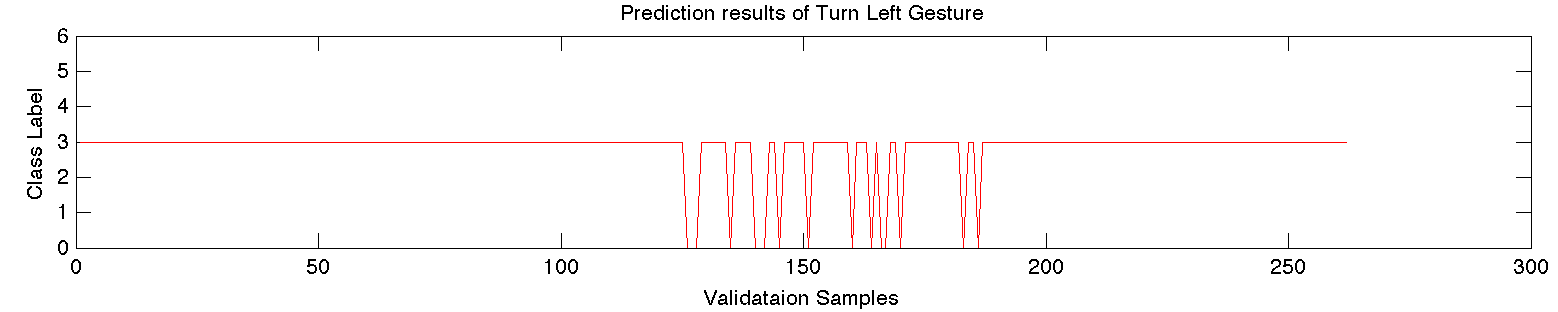
\includegraphics[width=150mm]{/result/test-prediction-turn-left.png} 
\end{figure}
\begin{figure}
	[h]
	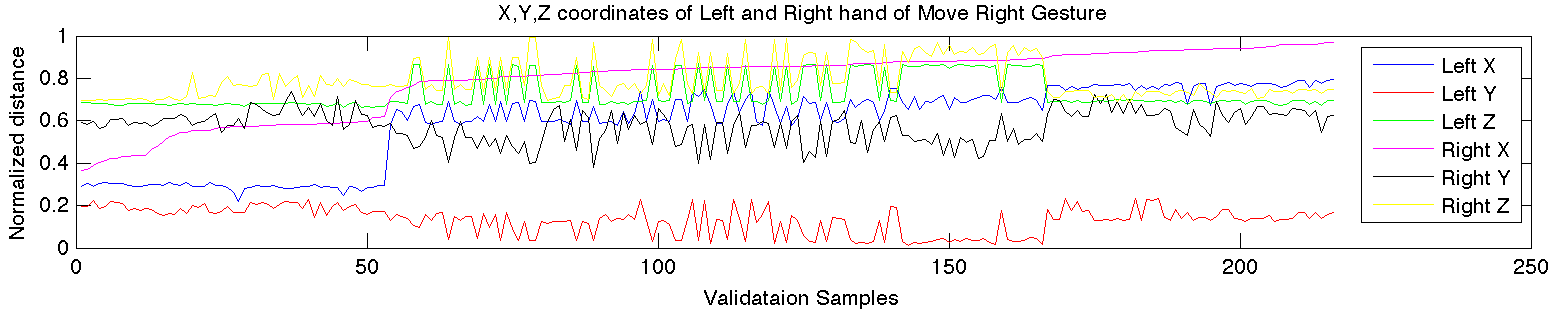
\includegraphics[width=150mm]{/result/test-axis-move-right.png} 
\end{figure}
\begin{figure}
	[h]
	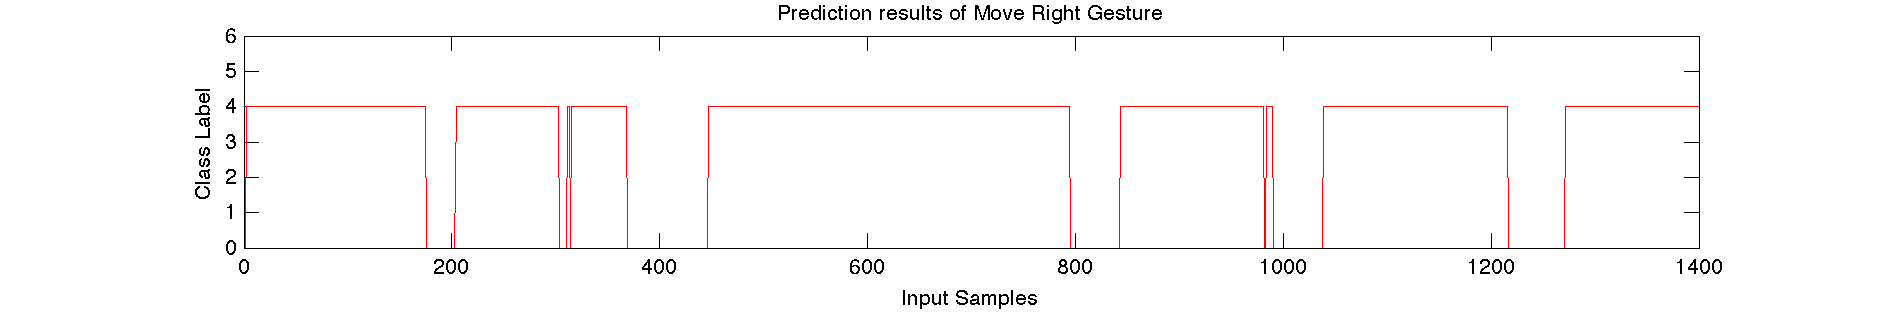
\includegraphics[width=150mm]{/result/test-prediction-move-right.png} 
\end{figure}
\begin{figure}
	[h]
	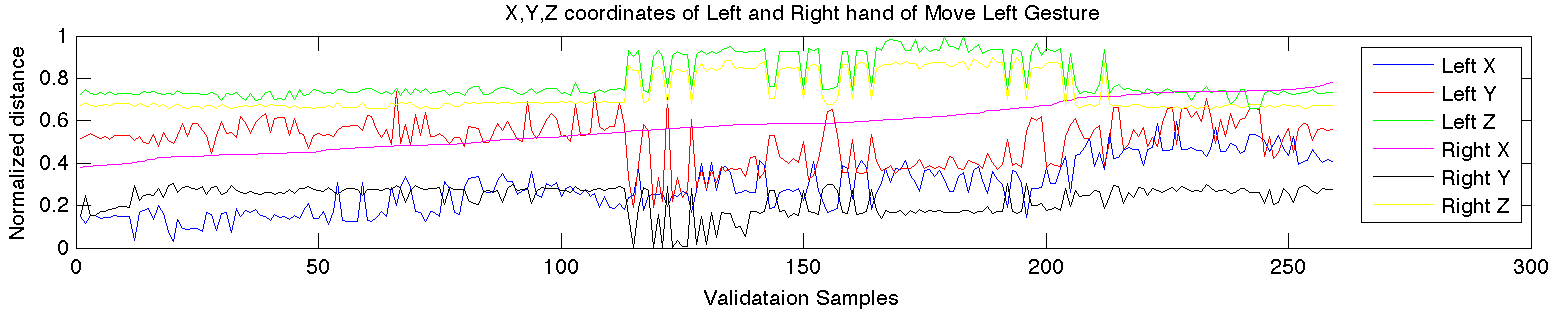
\includegraphics[width=150mm]{/result/test-axis-move-left.png} 
\end{figure}
\begin{figure}
	[h]
	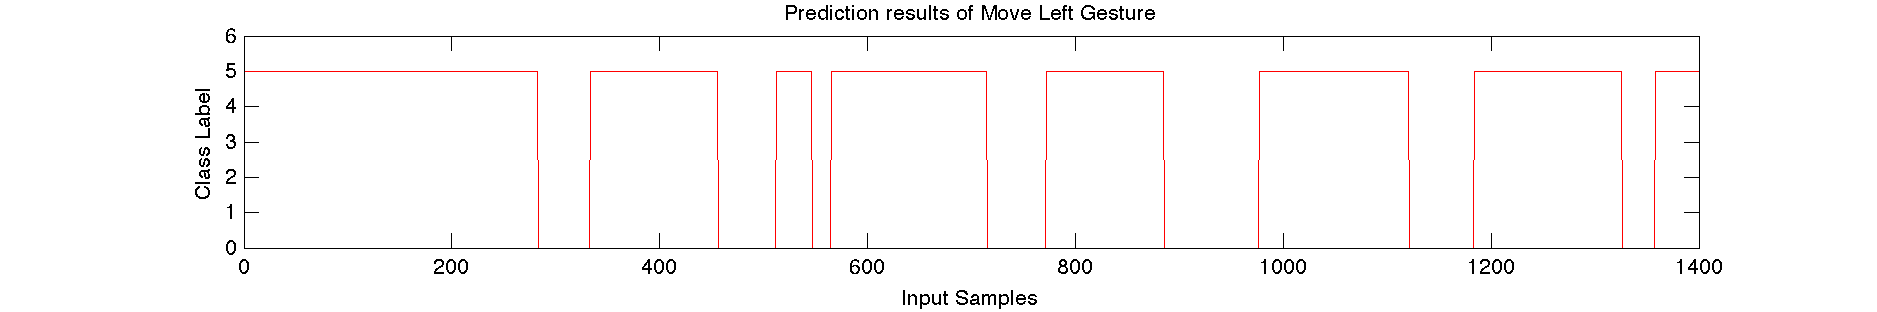
\includegraphics[width=150mm]{/result/test-prediction-move-left.png} 
	\caption{Prediction results of test data.}
	\label{ev:test:prediction}
\end{figure}

\begin{figure}
	[h]
	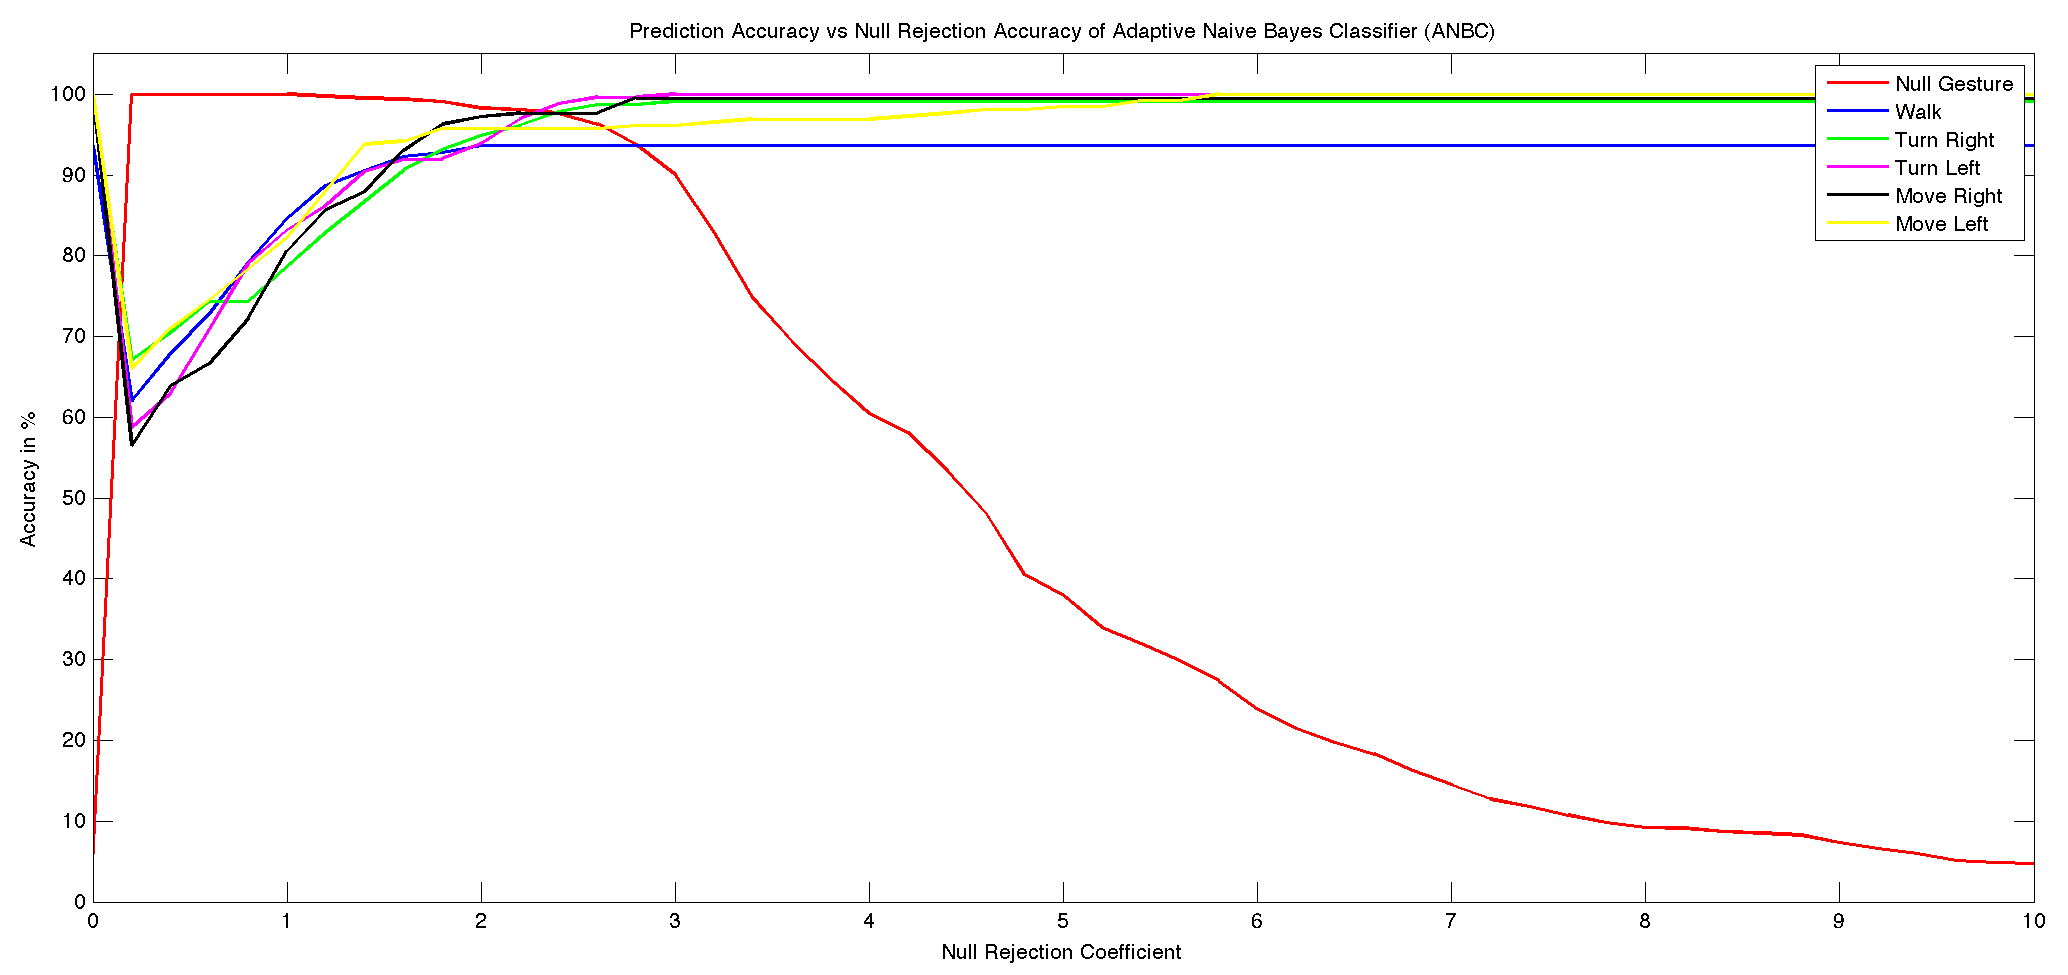
\includegraphics[width=150mm]{/result/test-accuracy-anbc.png}
	\caption{Prediction vs Null Rejection of ANBC}
	\label{ev:accuracy:anbc}
\end{figure}
\begin{figure} 	
	[h]
	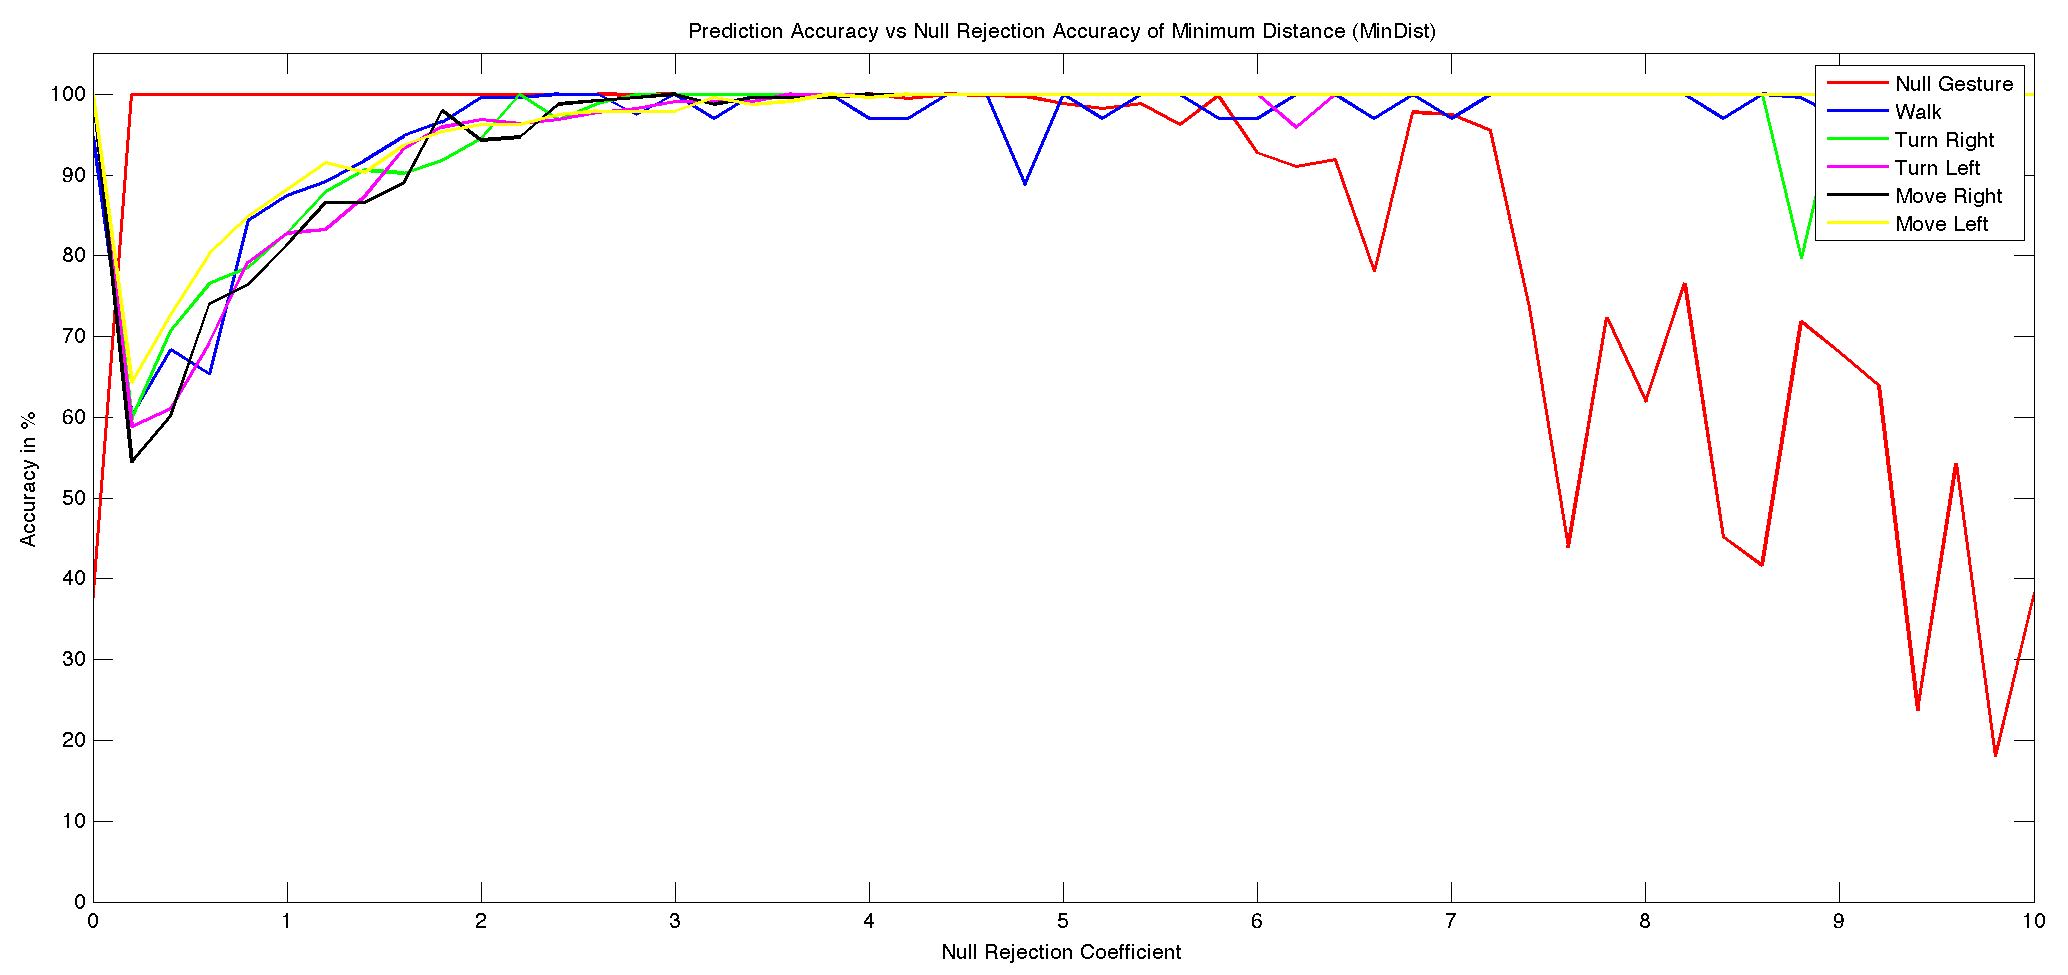
\includegraphics[width=150mm]{/result/test-accuracy-mindist.png}
	\caption{Prediction vs Null Rejection of MinDist}
	\label{ev:accuracy:mindist}
\end{figure}